\section{Difficulty Modeling Imhibition}

\subsection{Main problem now}
When we solve the system of linear equations, more than one row can be zeros.

This problem rarely occurs when there is a larger pressure difference between the top and bottom row of nodes. Rarely because it is possible to have a subsystem even when there is a significant pressure difference between the top and bottom nodes, where the system of linear equations have infinitely many solutions. 


\subsection{The flow does not start in the nodes}

The flow did not start when all the meniscus were located inside the nodes. Because in our model we assumed that there is not capillary pressure in the nodes. To overcome this, the meniscus were made to be situated inside the tubes.

\subsection{The flow does not start, all meniscus midway in thick tubes}

The solution of linear equation were such that, the capillary force balanced out the pressure gradient. The pressure was much higher outside in the thick tubes than in the thin tubes. [NEED TO VERIFY] whether this was caused by error in the process of solving the linear equation or due to the initial setup, needs to be checked again. Error is, that it is impossible to determine whether the coefficient during the process of gauss elimination is zero or not. Because of the way how floating point numbers are handled by the CPU, 0 is often seen as a small number, for example 

\section{Description of the Model}
	The algorithms and methods used to simulate two-phase flow in porous media has many practical applications in oil recovery, hydrology, electricity production where pressurized water is passed through heated pipes and is transformed into steam, etc. Our algorithm presented here is used to find the saturation of a phase with respect to time, the hysteresis curve when the pressure across the porous body is reversed, total capillary pressure as a function of saturation[4], and determination of permeability which appears in Darcy’s law.

	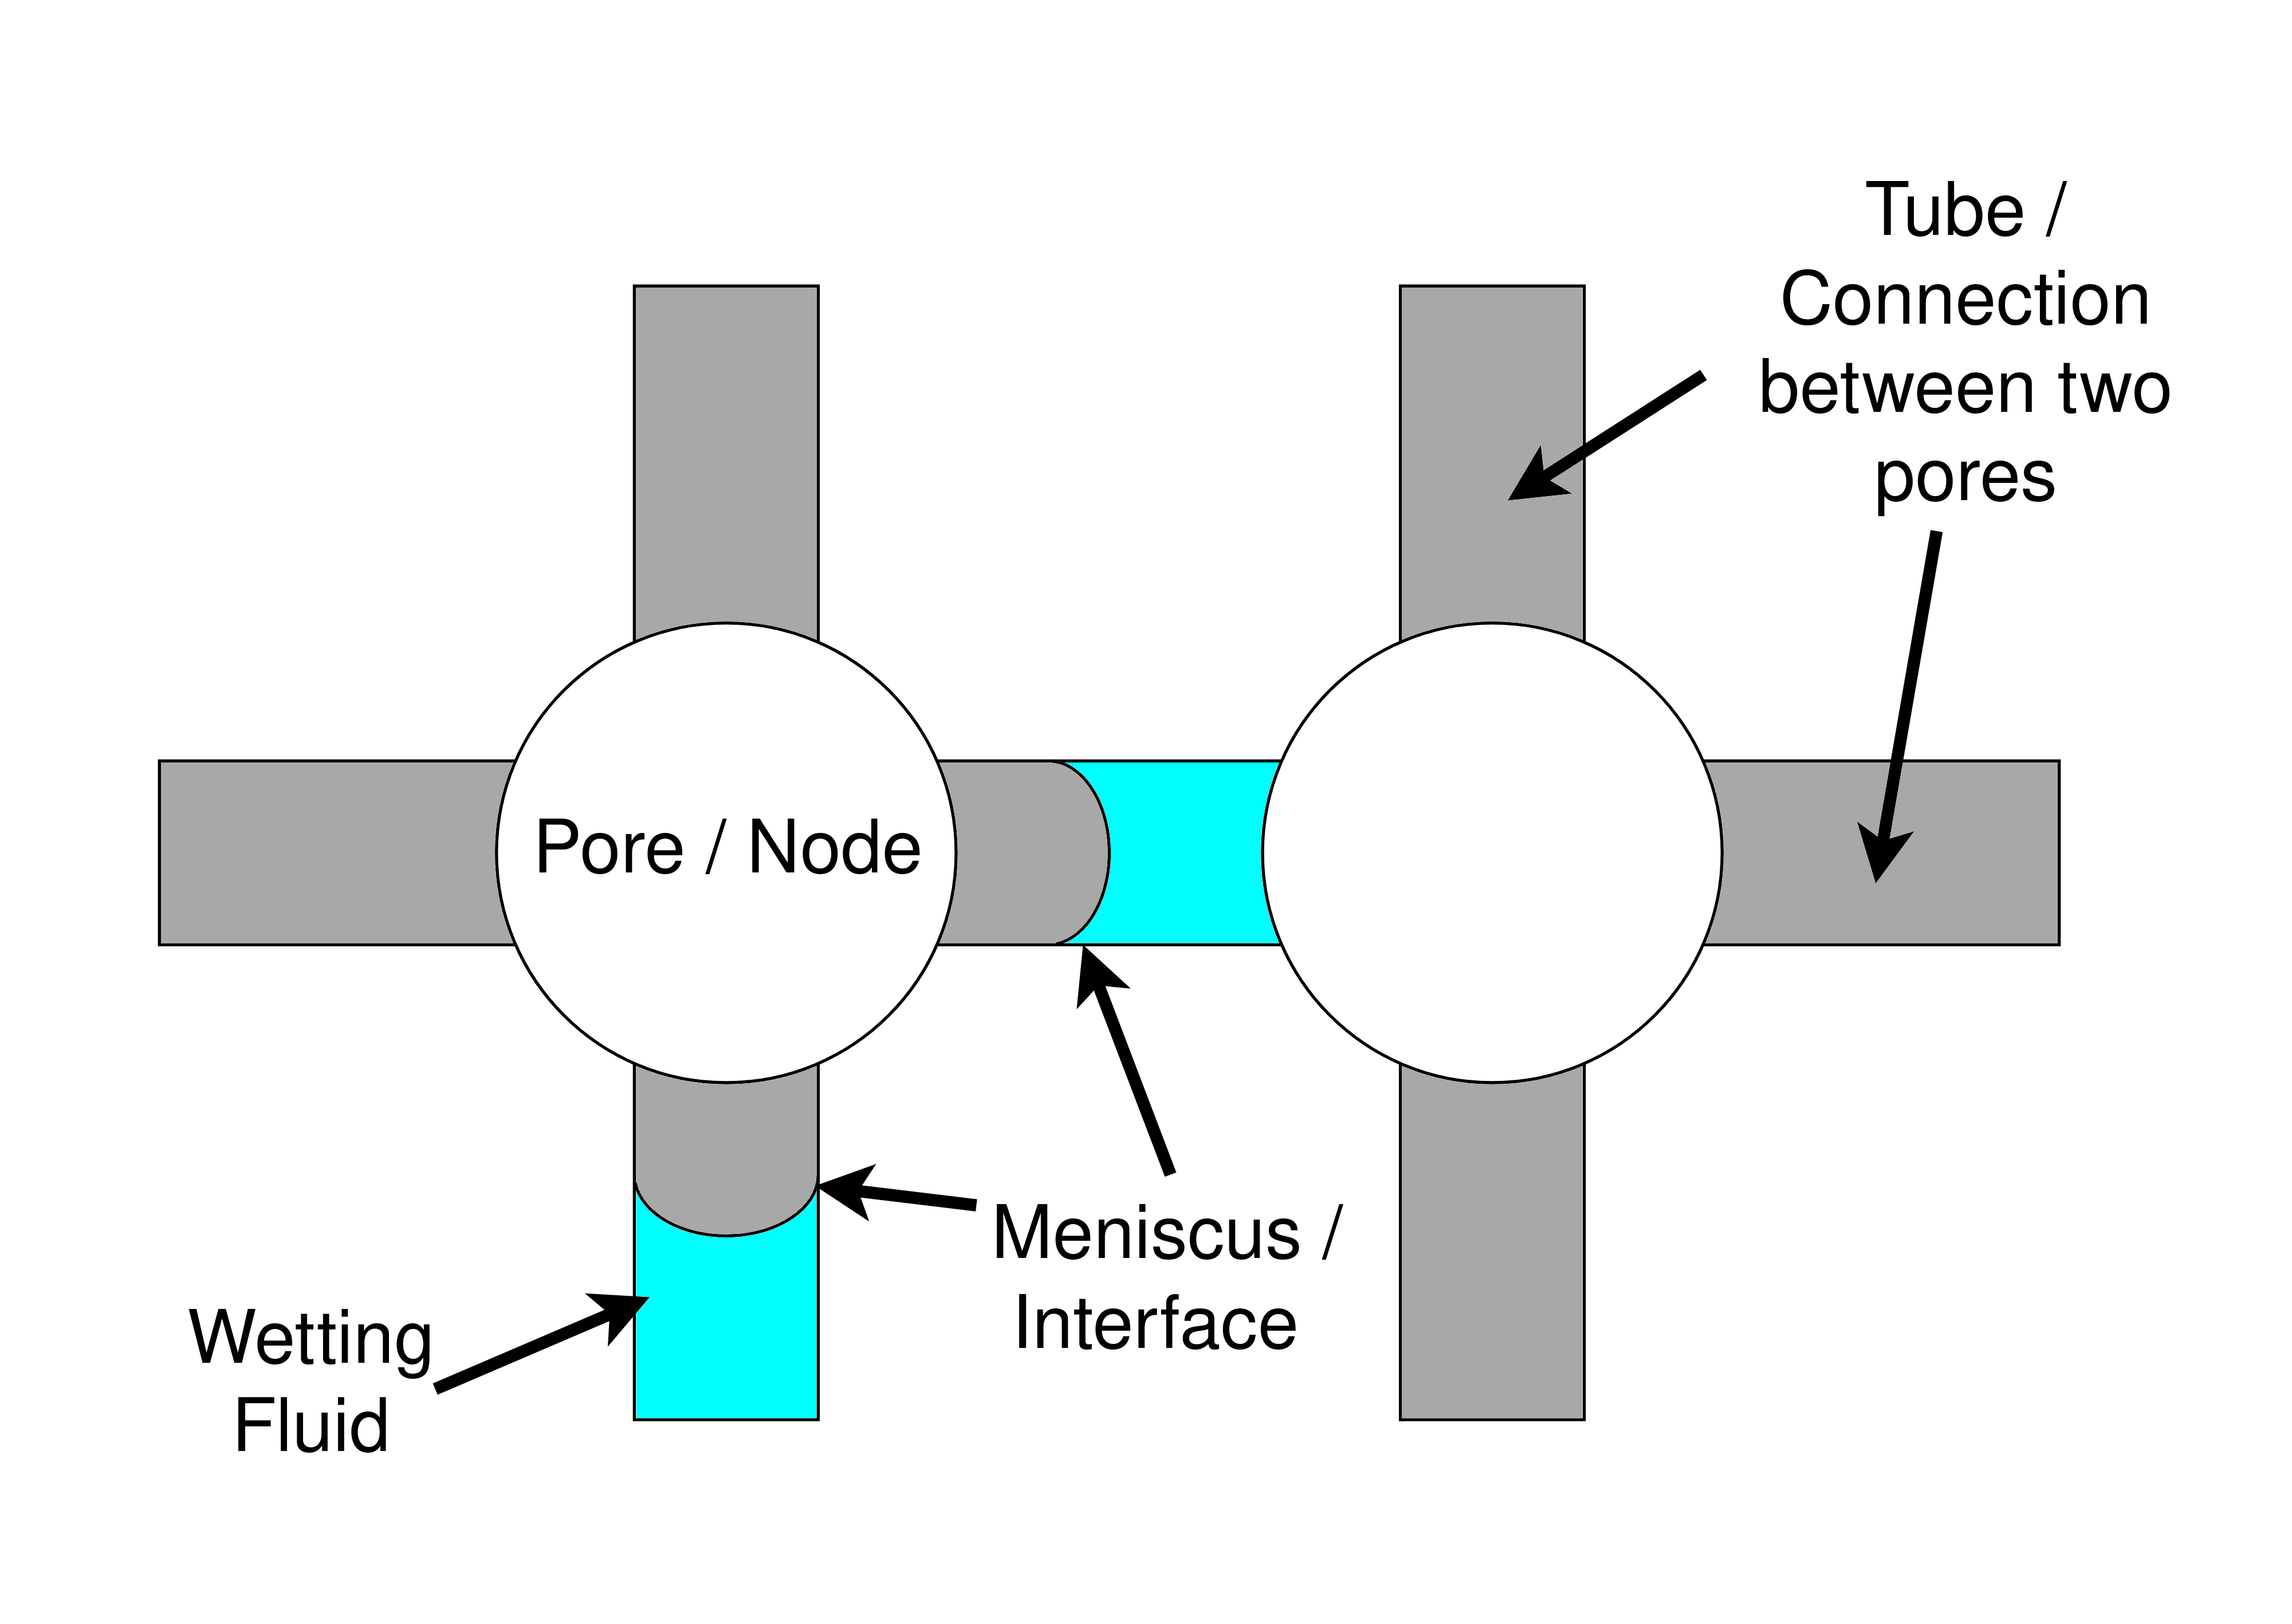
\includegraphics[height=6cm]{fig_descp-of-model}
	
	Figure showing two nodes from the network where the size of the node is much larger than the radius such that the capillary force tends to zero when the meniscus enters a node. 

\section{Algorithm steps !UNDER CONSTRUCTION}
	\begin{enumerate}
		\item \textbf{Input Files:} read input files, radius.txt and mns.txt, mns.txt contains the initial setup of the meniscus
		\item \textbf{Random radius:} add very small random values to the radius, this is done in order to remove the case of two equal radius for simplicity, can be removed later
		\item \textbf{Loop time:} do until a certain proportion of invading fluid is reached for example 0.90:
		\begin{enumerate}
			\item \textbf{Pressure:} determine the pressure at each node using the linear equations given in section \ref{sec:linear-equ}.
			\item \textbf{Velocity:} Calculate the velocity using equation \ref{eq:velocity-in-tube} 
			\item \textbf{time step:} determine the time step, the time step is calculated such that, it is the minimum of the time taken for a meniscus to reach a node it is heading towards. It is calculated by iterating through all the tubes, for a tube the time is determined using the $t_{ij} = x_{ij} / v_{ij}$, here $x_{ij}$ is the distance between the node and and the meniscus closest to it, if the fluid is traveling upwards then it is the node located on the top of the tube, if the velocity is downwards then the node which is at the bottom is used. In case there is no meniscus present, $x_{ij} = l_{ij} / 4$ is used, it is because a meniscus can enter the tube during the time step and this meniscus must not reach the next node, it can happen if the velocity is high and the radius is small. Also if $x_{ij} > l_{ij} / 4$, then $x_{ij} = l_{ij}/4$ is used. This is done in order to smoothen the integration. In the video $l_{ij}/4$ is used, the number can be increased.
			\item \textbf{volume:} The volume displaced in each tube is determined by iterating through all the tubes, $V_{ij} = v_{ij} * t_{min}$.
			\item \textbf{integration:} 
				\begin{enumerate}
				\item \textbf{Store insertion:} create a matrix to store how much of which fluid to insert in each of these tubes.
				\item \textbf{Loop nodes:} Iterate through all the nodes, and for each of the nodes. 
					\begin{enumerate}
						\item divide the tubes into two categories, flow-in-tube - here the fluid from these tubes flow into the nodes, flow-out-tubes here we insert the fluid into the tube from the node
						\item Find out the total of fluid1, fluid2, which is the total of each fliud from all flow-in-tubes.
						\item Start filling the each of the flow-out-tubes where the flow will go into in ascending order of the radius of the tube. This will be done simply be adding the quantity of fluid1 and fluid2 to the matrix created above.
						\item while filling fist use fluid1, once fluid1 is used up then start using fluid2, which means if in a tube we have to insert two fluids, then fluid1 will go in first.
					\end{enumerate}
				\item \textbf{Fluid addition:} For each of the tubes, add the volume of fluid determined to be added. After addition if there are more than 2 meniscus, then merge them retaining their center of masses.
				\end{enumerate}
			\item \textbf{Picture:} Save a picture of the current configuration.
			\end{enumerate}
		\item {Video:} Make a video file from the pictures.
	\end{enumerate}
